
\msection{Distributed Processing (Objective 1)}
\label{sec:aim1}

Recent work in machine learning has studied the effect of
communication constraints and parallelization in distributed
estimation. There is a close parallel in vision, where any given input
is sensed by multiple parts of the retina and an accurate percept
needs to be constructed. We will consider different models
for distributed processing, motivated by learning and perception in
both lower-level organisms (visual processing in fruit flies) and
higher-level cognition (visual cognition in humans). 


\biobackground{}
Animals use visual cues to guide many behaviors, from navigation to
foraging and courtship. The perception of these visual cues is an
inference problem \citep{knill:96}. In this problem, the
animal obtains light intensity information from an array of
photoreceptors focused on different points in space. The animal must
combine these light intensity signals in a way that allows it to infer
and respond the true state of the world, across many different
parallel dimensions of inference. For instance, one dimension of
inference might be the global motion of the visual scene, while
another might be the existence or non-existence of a predator in the
scene. The neuronal circuits in the visual system perform this
inference task, at both low levels (is there an edge at this location
and angle?) and at high levels (is that object a predator?)
\citep{simoncelli:01}. The operational processing of many
visual neurons and circuits have been studied in depth, but it is
frequently unknown how these operational descriptions relate to the
inferences that guide behavior. In particular, these inferences
require integrating distributed retinal information over space and
over time, but we do not know how this integration relates to the
statistics of the natural world, to channels of information flow
within the circuits, or to noise or incomplete information about the
world.

The fruit fly \textit{Drosophila} has several advantages for studying the
distributed visual processing that guides perception and
behavior. First, there is a powerful genetic toolbox in fruit flies
that allows researchers to genetically define, manipulate, and monitor
specific classes of neurons \citep{luo:08}. Those manipulations
also allow specific neurons to be causally connected to
behaviors. Second, the fly has a wealth of robust visual behaviors,
including regulation of turning and speed, escape responses, and
courtship behaviors \citep{card:08,silies:14,spieth:74}.
Third, the field has identified neuron types that
appear to be making exactly the inferences described above: neurons
sensitive to local motion direction and speed \citep{Maisak:13};
neurons sensitive to wide-field motion that corresponds to rotational
self-motion of the fly about various axes \citep{joesch:08};
neurons sensitive to looming (approaching) dark
dots \citep{devries:12,klapoetke:17}; and neurons sensitive to
moving small dots \citep{keles:17}. In each of these cases, we
can silence the neurons and observe behavioral deficits. We can also
record neural activity in these individual neurons and measure their
response properties with well-controlled visual stimuli
\citep{salazar:16}. Thus, these neuron classes act as
handles for understanding how visual inferences are made, and how
neurons extract specific visual features from a spatiotemporally
distributed set of inputs.


\setlength{\columnsep}{20pt}
\begin{wrapfigure}{R}{0.45\textwidth}
\centering
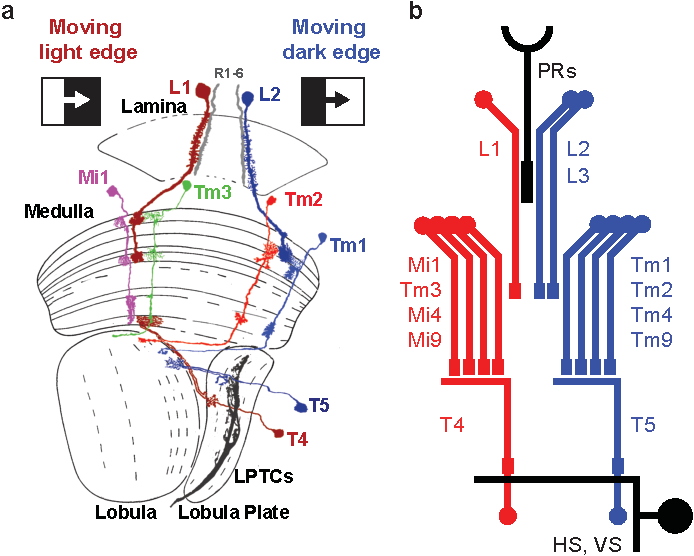
\includegraphics[width=.44\textwidth]{figs/flysetup}
\caption{\small Motion circuits in the fly. (a) Light is detected at the
retina (at the top of this diagram), and information is processed
moving down through different neuropils. Each of the highlighted
neurons is required for motion detection. Motion detection is split into one circuit that
detects light edges moving over dark backgrounds and another that
detects dark edges over light backgrounds. (b) Cartoon of
neurons known to be involved in motion detection in the light edge
(red) and dark edge (blue) pathways. 
There are four T4s and four T5s, selective for each
of the four cardinal directions across the retina. This circuit repeats at all
points in space.}
    \label{fig:setup}
    \vskip2pt
\end{wrapfigure}

\statbackground{}
Statistical theory studies the difficulty of estimation under
various models, and attempts to find the optimal estimation
procedures.  Such studies usually assume that all of the collected
data are available to construct the estimators.  Recent research
has begun to study the problem of statistical estimation with data
residing at
multiple machines.  Estimation in distributed settings is becoming
common in modern data analysis tasks, as the data can be collected or
stored at different locations.  In order to obtain an estimate of some
statistical functional, information needs to be gathered and
aggregated from the multiple locations to form the final
estimate. However, the communication between machines may be
limited. In such a setting, it is important to understand how the
statistical risk of estimation degrades as the communication budget
becomes more constrained.

The so-called CEO problem, first studied in the EE 
community in the context of rate-distortion-theory theory, treats a
similar distributed estimation problem \citep{berger1996ceo,
  viswanathan1997quadratic}.  Recently, several studies have
focused on more specific statistical tasks and models, including mean
estimation, regression, principal eigenspace estimation, and discrete
density estimation \citep{zhang2013information, shamir2014fundamental,
  battey2015distributed, braverman2016communication,
  diakonikolas2017communication, fan2017distributed,
  lee2017communication, shang2017computational}. Most of this existing
research treats parametric and discrete models, where the
parameter of interest has finite dimension.  In a nonparametric
setting, the effective dimension of the problem typically grows with
the sample size, and these results no longer apply.
Other results have been obtained on these problems in the normal means
model of nonparametric estimation, which arises naturally when representing an estimator in terms of an
orthogonal
basis \citep{johnstone2002function,tsybakov:2008}.  One
result gives a sharp constrained minimax analysis of nonparametric
regression under quantization constraints \citep{Zhu:18}; another
characterizes lower bounds and achievability for distributed
nonparametric regression \citep{Zhu:18b}. Similar results have been obtained 
using wavelets and Besov spaces \citep{szabo18}.


\project{Parallel channels for local motion detection}
The fly's eye is arranged in a hexagonal lattice of repeated circuit
motifs, with each column of circuitry representing one retinotopic
point in visual space. Each eye consists of an array of roughly 800 of
these pixels, which together cover approximately one half of visual
space. Two classes of local motion detection cells exist in every
column: there are T4 cells, which detect light edges moving across
dark backgrounds, T5 cells, which detect dark edges moving across
light backgrounds. There are 4 of each class, one for each cardinal
direction. Thus, there are 8 parallel channels at each point in space
representing motion in two dimensions. Why is the system organized in
this way? How are naturalistic motion signals distributed across the 8
channels, and what encoding or decoding advantages does this serve?
Under what conditions are the channels redundant? How would an optimal
observer partition signals among these parallel channels? Could a data
driven approach predict or give insight into this encoding scheme?
One approach to begin studying these questions will be to adapt
the classical framework of sparse coding \citep{Olshausen:Field:96}
in a way that represents the neurobiology of the fly's visual system.

\project{Detecting motion flow fields}
When an animal moves or rotates in the world, its
self-motion generates flow fields across its retina. These flow fields
are often used as feedback to control orientation or speed.
In \textit{Drosophila}, some neurons downstream of the local motion
detectors have large receptive fields that integrate motion signals
across the retina. They appear to be selective for specific flow
fields, which correspond to the flow fields created by the rotation of
the fly about different axes. These neural signals have been proposed
to be linear filters, matching their weighting for local motion to
specific optical flow fields (``matched filters''). However, it is not
clear whether a linear weighting of local motion estimates represents
a best estimate of each flow field, or whether more complex dendritic
computations could improve encoding. In particular, it is not clear
how these neurons might optimally integrate motion signals in the
presence of occlusions or differential velocity fields that would be
caused by fly translation through space. We will investigate these
issues using methods based on hierarchical sparse coding 
\citep{Yu:2011} and related computational methods for
low rank decomposition.


\setlength{\columnsep}{10pt}
\begin{wrapfigure}{l}{0.45\textwidth}
\centering
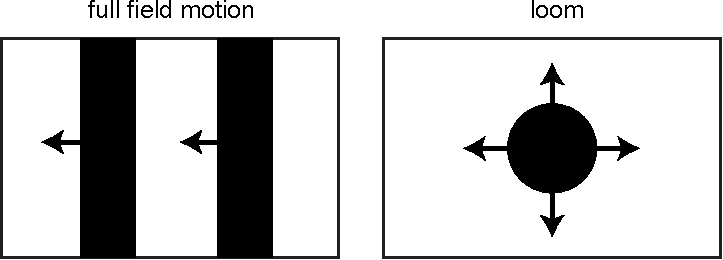
\includegraphics[width=.44\textwidth]{figs/loom}
\caption{\small Global motion and loom may generate similar local
motion signals, but local motion signals must be integrated over space
to distinguish the two stimulus types.}
    \label{fig:loom}
\vskip-2pt
\end{wrapfigure}

\project{Detecting looming stimuli}
Looming stimuli are created by objects as they approach the observer:
the object becomes larger, and if it is on a collision course,
opposite edges of the object will move in opposite directions on the
retina. Thus, detecting loom requires integrating information over
space, as any local motion detector cannot know if local motion is due
to a looming object or is just wide-field motion. Two neuron types in
\textit{Drosophila} have recently been described as loom detectors,
responding selectively to objects that grow larger in their receptive
fields. The receptive fields of these cells to local motion have been
characterized, but the relationship between these receptive fields,
the nonlinear computations of these neurons, and the statistics of
natural loom stimuli remain unclear. This is in large part due to the
absence of good statistics on natural loom stimuli. It is also
possible that these loom detectors use features beyond motion to
detect approaching objects; for instance, a detector might integrate
motion signals with light intensity information, since light intensity
is correlated with distance. Here, one might also ask whether the
motion detecting neurons upstream of the loom-sensitive neurons could
convey information about stimulus features beyond just motion
direction and speed. We will abstract loom detection as a statistical
testing problem, building on work such
as \citep{castro:05,huo:06,hc:04}.  Specifically, for a given object
geometry such as a disk, we will study minimax rates for loom
detection, in terms of the noise level and sparsity of the number of
boundary neuron measurements required. Fast hierarchical algorithms
to achieve the minimax rates will be studied.



